\documentclass{beamer}

\usetheme{metropolis}

\usepackage[latin1]{inputenc}
\usepackage{amsmath,amssymb}
\usepackage{subcaption}
% \usepackage{enumitem}

% \setlength{\leftmargini}{0pt}
% \setlength{\leftmarginii}{0pt}
% \setlength{\leftmarginiii}{0pt}

\usepackage[style=verbose]{biblatex}
\addbibresource{cit.bib}

\newcommand\oneline[1]{\resizebox{\linewidth}{!}{#1}}

\newcommand\figvs[1]{
  \begin{figure}
    %
    \center
    %
    \begin{subfigure}{.45\textwidth}
      %
      \centering
      %
      \includegraphics[width=\linewidth]{{#1.flout}.pdf}
      %
      \caption{Force-Directed}
      %
    \end{subfigure}
    %
    \begin{subfigure}{.45\textwidth}
      %
      \centering
      %
      \includegraphics[width=\textwidth]{{#1.hdpca.12}.pdf}
      %
      \caption{HD Embedding}
      %
    \end{subfigure}
    %
  \end{figure}
}

\newcommand\figtab[1]{
  \begin{figure}
    %
    \center
    %
    \begin{tabular}{cccc}
      $1^{st} PC$ & $2^{nd} PC$ & $3^{rd} PC$ & $4^{th}$ PC \\
      &
      \includegraphics[width=.22\textwidth]{{#1.hdpca.12}.pdf} &
      \includegraphics[width=.22\textwidth]{{#1.hdpca.13}.pdf} &
      \includegraphics[width=.22\textwidth]{{#1.hdpca.14}.pdf}\\
      & &
      \includegraphics[width=.22\textwidth]{{#1.hdpca.23}.pdf} &
      \includegraphics[width=.22\textwidth]{{#1.hdpca.24}.pdf}\\
      & & &
      \includegraphics[width=.22\textwidth]{{#1.hdpca.34}.pdf}
    \end{tabular}
    %
  \end{figure}
}

\title{\oneline{Qualitative Discovery of Marine Population Trends}}
\date{}
\author{\textbf{Student:} Andrea Baisero \\ \textbf{Community Partner:} Benjamin Moran}

\begin{document}

\maketitle

\begin{frame}{Overview}
  \tableofcontents
\end{frame}

\section{Problem Description}


\begin{frame}{Problem Description}

  \begin{block}{Project Partner:}

    \emph{Benjamin Moran}, undergraduate Senior in Marine Biology.

  \end{block}

  \begin{block}{Data Description:}

    Sample statistics on various fish species obtained over the course of 20
    years in 3 regions: the Florida Keys, Dry Tortugas National Park, Southeast
    Florida Coral Reef Initiative (SEFCRI) areas.

  \end{block}

\end{frame}

\begin{frame}{Datasets}

  \begin{description}

  \item[Taxonomy:]  Biological hierarchy of family, genera, and species.

  \item[Samples:]  Histogram: \begin{itemize}

      \item Region, i.e. {\small (FLA KEYS, DRY TORT, SEFCRI)};

      \item Date;

      \item Location, i.e. latitude and longitude;

      \item Size, {\small (sometimes negative!!!)};

      \item Depth;

      \item Protection Status, {\small (location dependent)};

      \item Count, {\small (not always integer!!!)};

    \end{itemize}

  \item[Strata:]  {Info on sampling areas, e.g. grid sizes, prot. status}

  \end{description}

  \vspace{-.2cm}
  \begin{block}{Notes}

    1) Very big (samples.csv $\sim$1GB)
    
    2) Infested with missing fields, \emph{semantically wrong values} (!!!).

    3) Original data server has been offline for various weeks.

  \end{block}

\end{frame}


\begin{frame}{Problem Description}

  \begin{block}{Project Partner:}

    \emph{Benjamin Moran}, undergraduate Senior in Marine Biology.

  \end{block}

  \begin{block}{Visualization Needs:}

    Discover explanatory conditions for variations in sample statistics.
    
    \begin{description}

      \item[Dependent variables:]  size and abundance.

      \item[Independent variables:]  location, date, protection status, depth,
        distance from shore, and habitat type.

    \end{description}

  \end{block}

\end{frame}

\section{Design}

\begin{frame}{Design Goals}

  \begin{itemize}

    \item Visualize sample data on top of a geographic map.

    \item Filter data according to region, taxonomy, location, date, protection
      status, \dots \\
    $\Rightarrow$ Visualize, navigate, and select elements of taxonomy tree.

    \item In-detail views specific to selected filters, with appropriate
      within-view and inter-view comparison capabilities.

    \item Preliminary analysis via standard ML techniques (e.g. KDE for data
      density estimation, GP for data regression lines)

  \end{itemize}

\end{frame}

\begin{frame}{Design Overview}

  \centerline{
  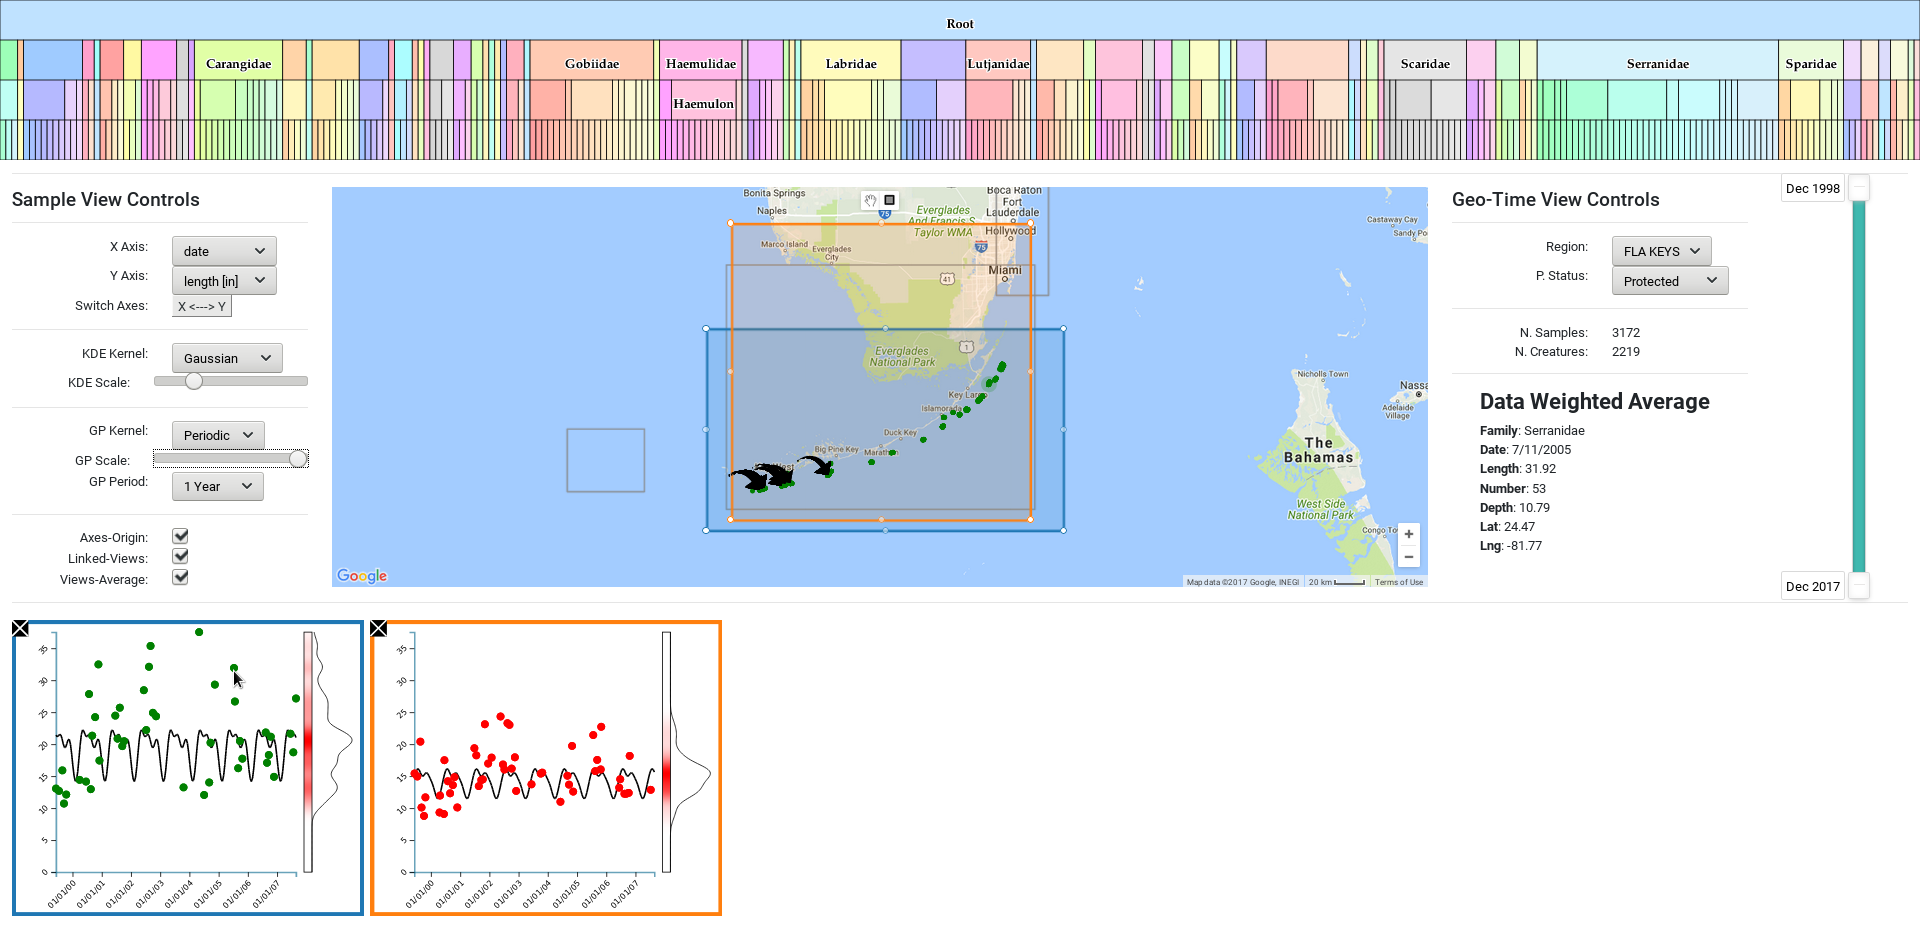
\includegraphics[width=\paperwidth]{./img/dviz.png}
  }

\end{frame}


\begin{frame}{Taxonomy Tree}

  \centerline{
  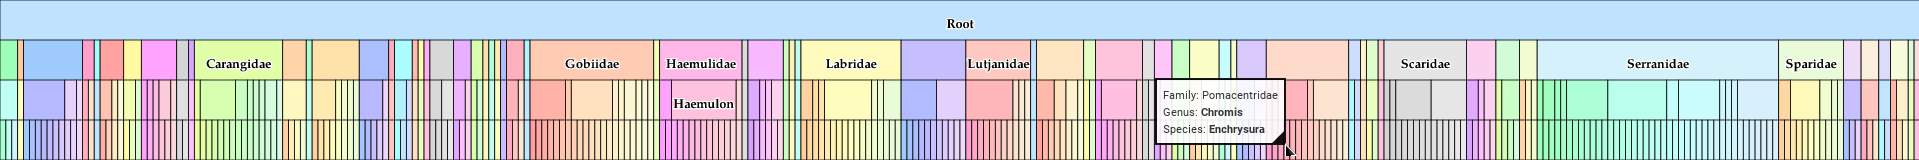
\includegraphics[width=\paperwidth]{./img/taxa.png}
  }

  \begin{description}

    \item[Goal:]  Show, navigate and select Family, Genus or Species.

    \item[Difficulties:]  Shallow, but high branching factor.

      Key concern:  space efficiency.

    \item[Solution:]  Inspired by Zoomable Sunburst\footcite{sunburst}, with
      key domain-specific changes.

      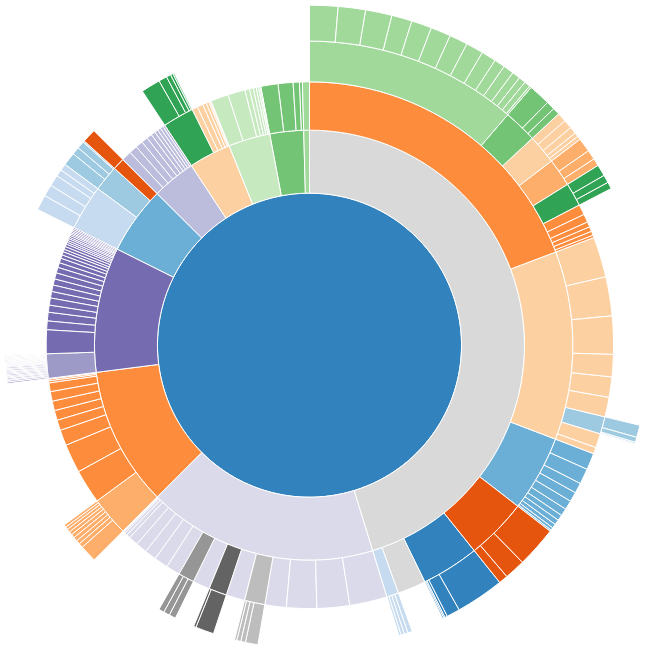
\includegraphics[width=.25\textwidth]{./img/taxa_sunburst.png}

  \end{description}

\end{frame}

\begin{frame}{Taxonomy Tree --  Visualization}

  \centerline{
  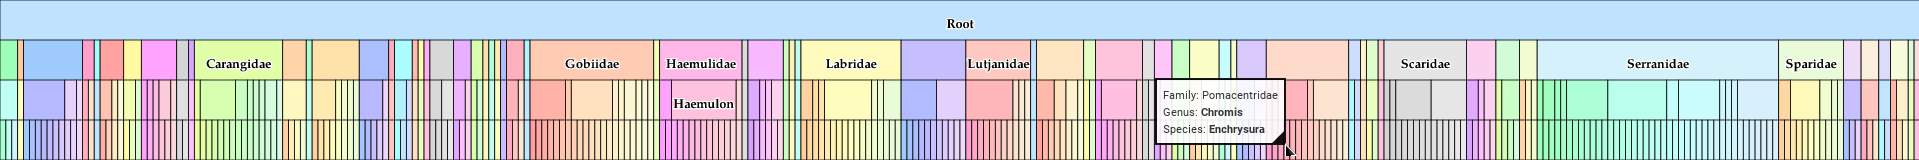
\includegraphics[width=\paperwidth]{./img/taxa.png}
  }

  Domain-specific features:

  \begin{itemize}

    \item Flattened out to exploit horizontal screen extension.
      
    \item Ordered hierarchically/alphabetically, to aid search.
      
    \item Labels only shown if sufficient space is available.

      {\small (More details available via tooltip + navigation)}

    \item Palette chosen to aide distinction between families
      
      {\small (small variations in hue applied to descendant genera/species)}

  \end{itemize}


\end{frame}

\begin{frame}{Taxonomy Tree -- Navigation and Selection}

  Clicking on an element\dots

  \centerline{
  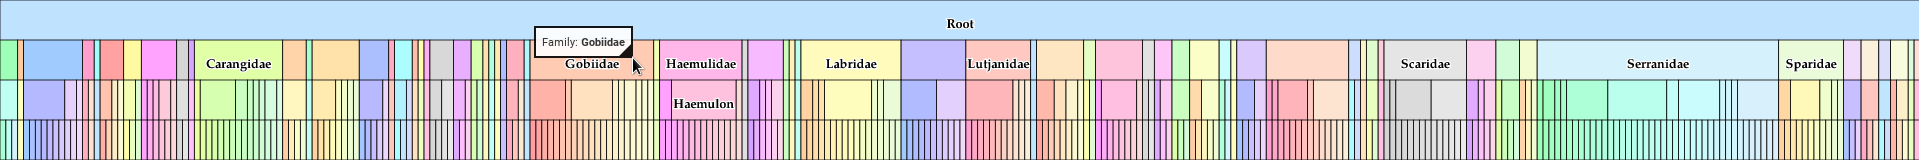
\includegraphics[width=\paperwidth]{./img/taxa_click.png}
  }

  \dots expands it, revealing new labels and allowing for tree navigation.

  \centerline{
  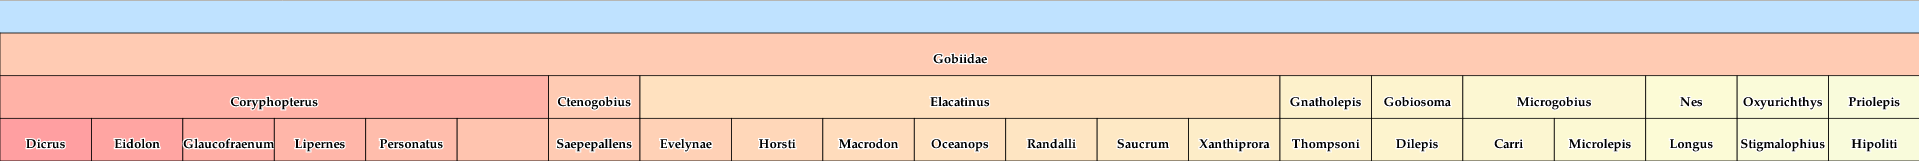
\includegraphics[width=\paperwidth]{./img/taxa_expanded.png}
  }

  Ctrl + click selects a family/genus/species for filtering purposes.

\end{frame}

\begin{frame}{Geographic View}

  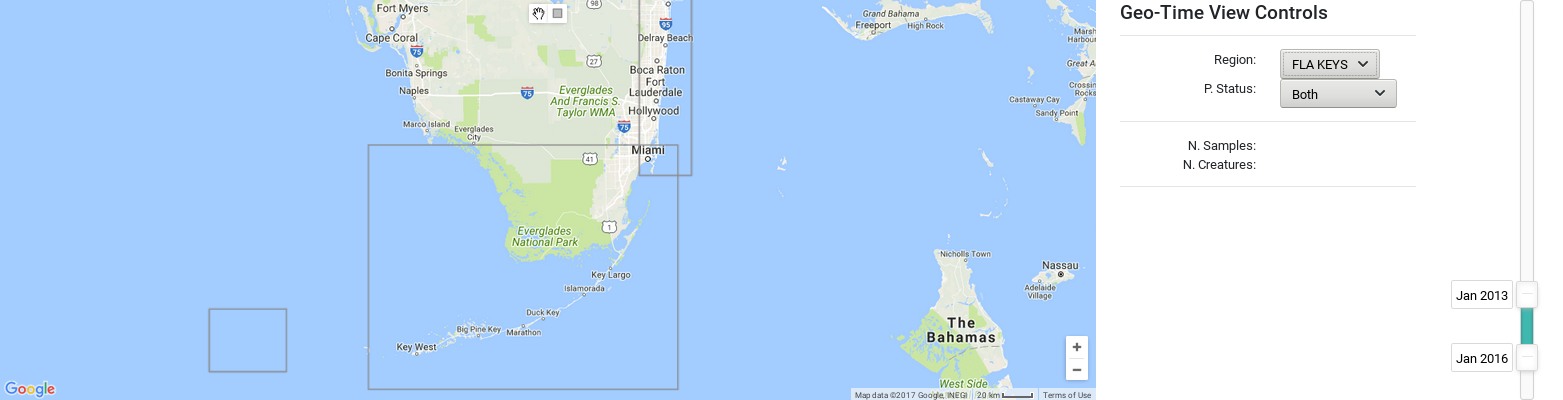
\includegraphics[width=\textwidth]{./img/geo.png}

  \begin{description}

    \item[Goal:]  Show, navigate and select by regions and area

    \item[Key Concern:]  Simple navigation (zooming, panning).

    \item[Solution:]  Based on Google Maps\footcite{gmapsapi}.
      
      \textbf{Pros}:  Many built-in functionalities {\small (zooming, panning,
      coordinates-to-pixel mappings)}.

      \textbf{Cons}:  Somewhat slow, and JS-blocking!!!

  \end{description}

\end{frame}

\begin{frame}{Geographic View -- Elements}

  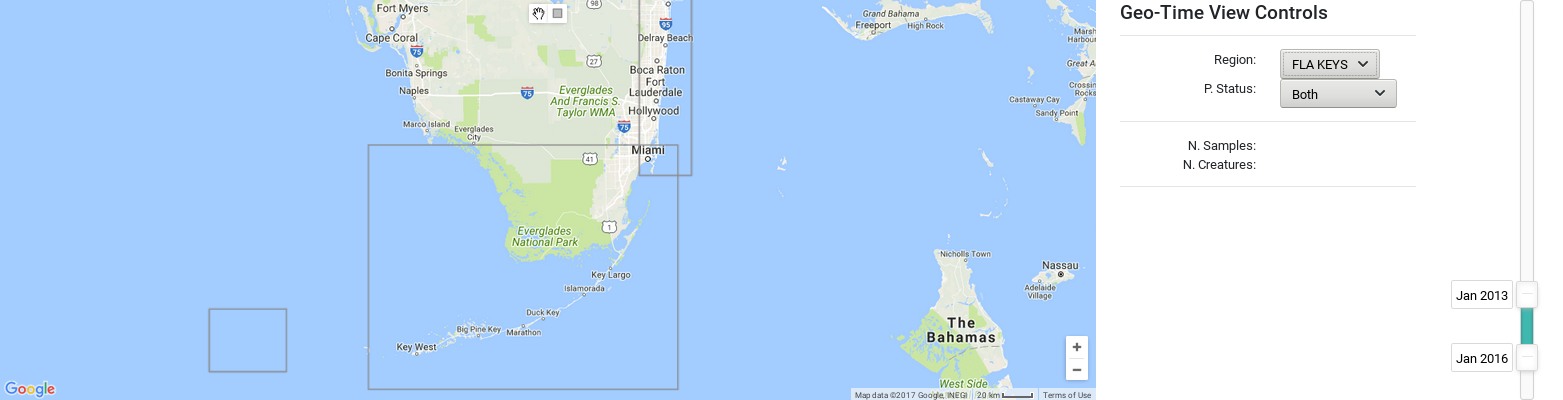
\includegraphics[width=\textwidth]{./img/geo.png}

  \begin{block}{Key Elements}
    
    \begin{itemize}

      \item Map

      \item Date Slider

      \item Region drop-down selection

      \item P. Status drop-down selection

      \item Empty space for labels + hover info

    \end{itemize}

  \end{block}

\end{frame}

\begin{frame}{Geographic View -- Examples}

  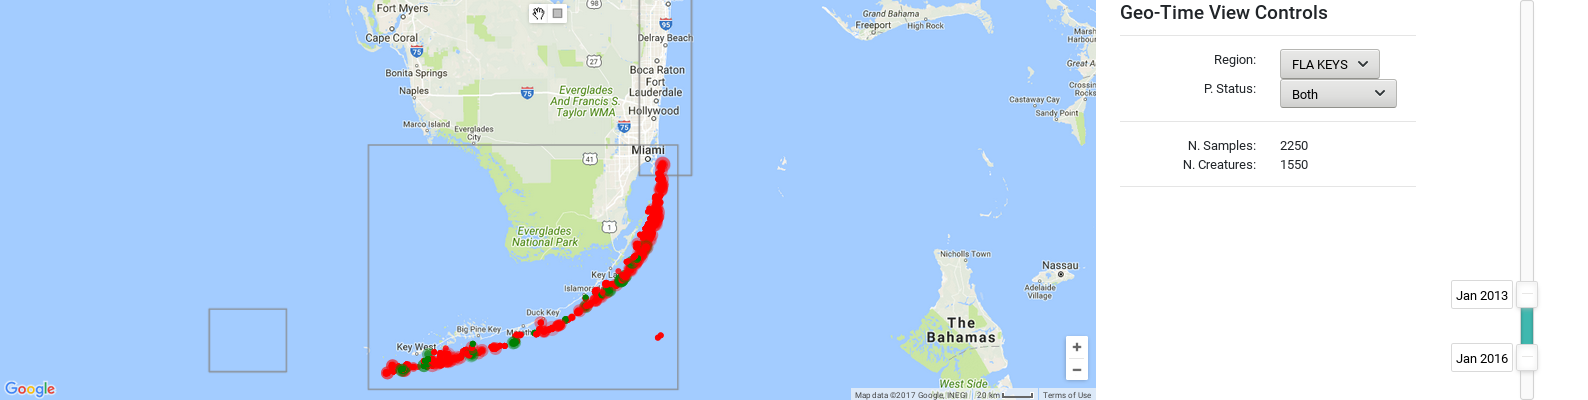
\includegraphics[width=\textwidth]{./img/geo_FLAKEYS_both.png}

  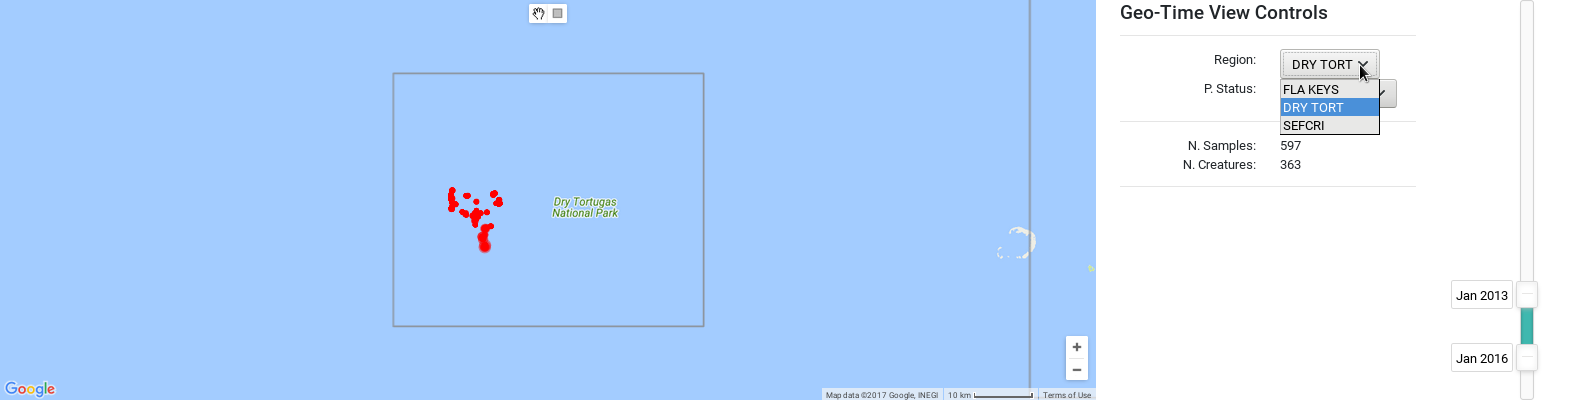
\includegraphics[width=\textwidth]{./img/geo_DRYTORT_nprot.png}

\end{frame}

\renewcommand{\footnotesize}{\scriptsize}

\begin{frame}{Detail Views}

  \centerline{
  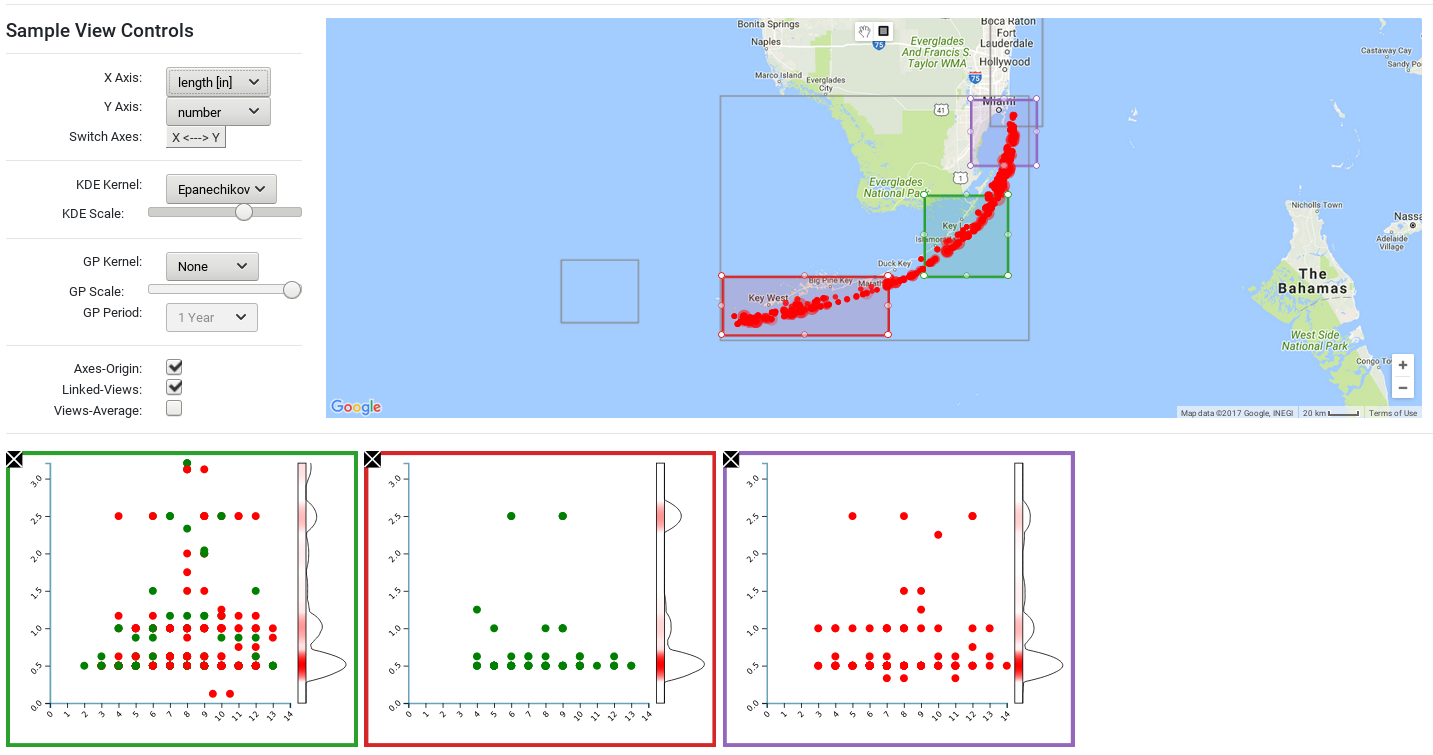
\includegraphics[width=.9\textwidth]{./img/fview.png}
  }

  \begin{description}

    \item[Goal:]  Maximum flexibility in view manipulation, (similar to ``From
      Detail to Overview'' and ``Glo-stix'').
      \nocite{van2014multivariate}\nocite{stolper2014glo}

    \item[Key Concerns:]  Maintaining data persistency.

      Ability to explore all sorts of potential relationships.

  \end{description}

\end{frame}

\begin{frame}{Detail Views -- Controls}

  \begin{block}

  \centerline{
    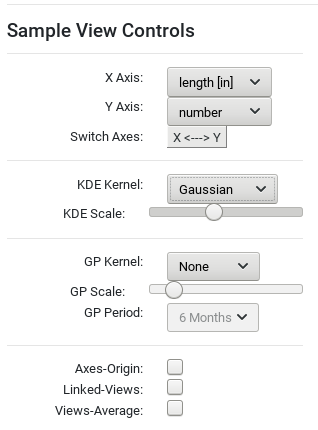
\includegraphics[height=3.5cm]{./img/fview_ctrls.png}
    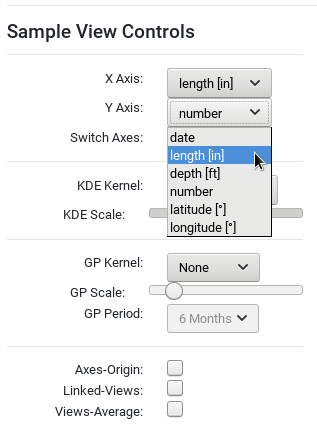
\includegraphics[height=3.5cm]{./img/fview_ctrls_yaxis.png}
    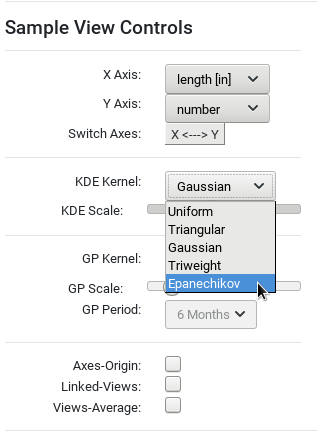
\includegraphics[height=3.5cm]{./img/fview_ctrls_kde.png}
  }

  \centerline{
    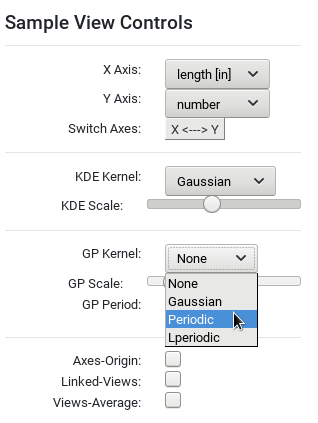
\includegraphics[height=3.5cm]{./img/fview_ctrls_gp.png}
    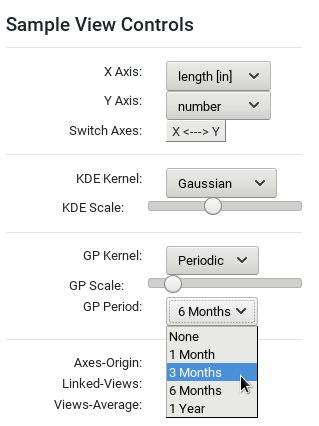
\includegraphics[height=3.5cm]{./img/fview_ctrls_gp_period.png}
    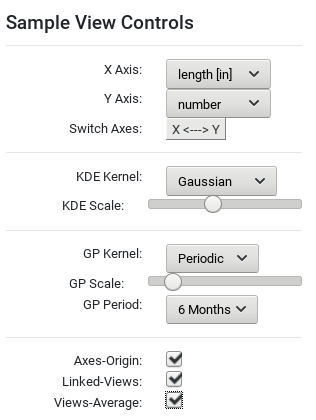
\includegraphics[height=3.5cm]{./img/fview_ctrls_checkboxes.png}
  }

  \end{block}

\end{frame}

\begin{frame}{Detail Views -- Avoiding Standard Plotting Biases}

  \begin{block}{Axis Origin:}

  \centerline{
  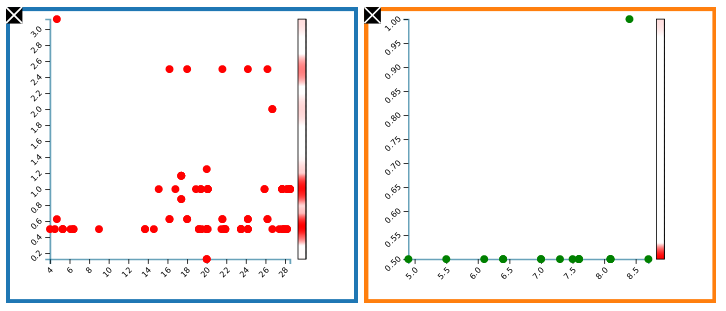
\includegraphics[height=2.35cm]{./img/fview_origin_pre.png}
  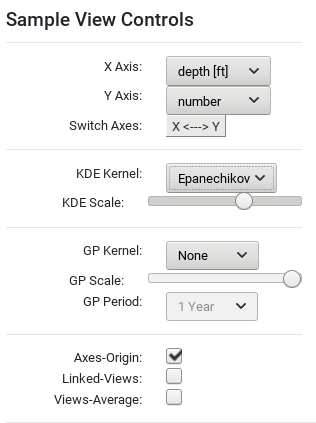
\includegraphics[height=2.35cm]{./img/fview_ctrls_origin.png}
  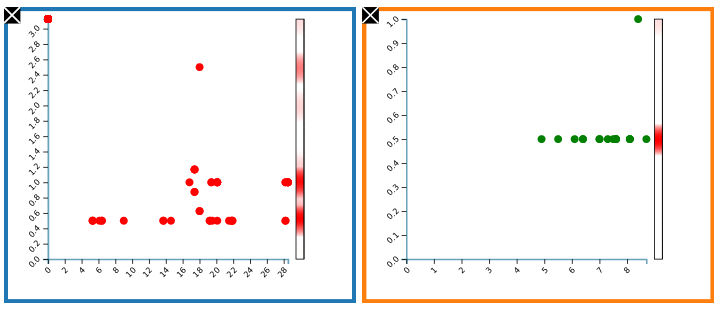
\includegraphics[height=2.35cm]{./img/fview_origin_post.png}
  }

  \end{block}

  \begin{block}{Linked Axes:}

  \centerline{
  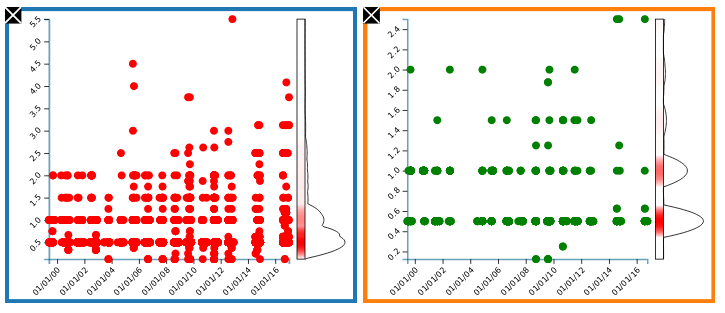
\includegraphics[height=2.35cm]{./img/fview_link_pre.png}
  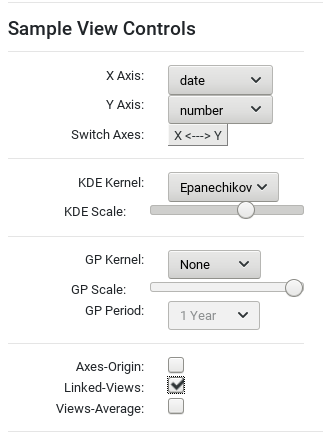
\includegraphics[height=2.35cm]{./img/fview_ctrls_link.png}
  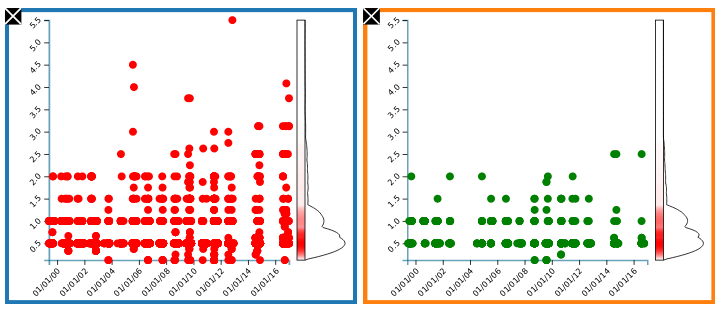
\includegraphics[height=2.35cm]{./img/fview_link_post.png}
  }
  
  \end{block}

\end{frame}

\begin{frame}{Detail Views -- Averaging over Sample Y-Axis values}

  \centerline{
  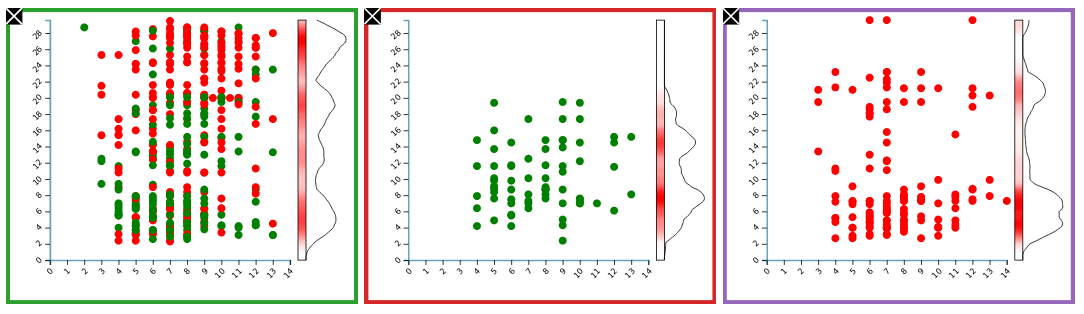
\includegraphics[height=2.35cm]{./img/fview_davg_pre.png}
  }

  \centerline{
  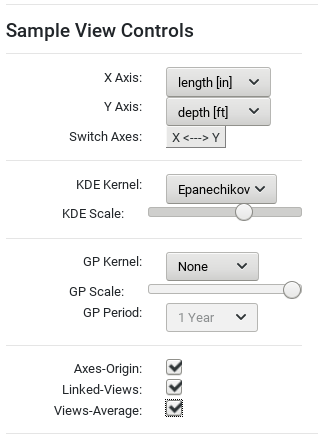
\includegraphics[height=2.35cm]{./img/fview_ctrls_davg.png}
  }

  \centerline{
  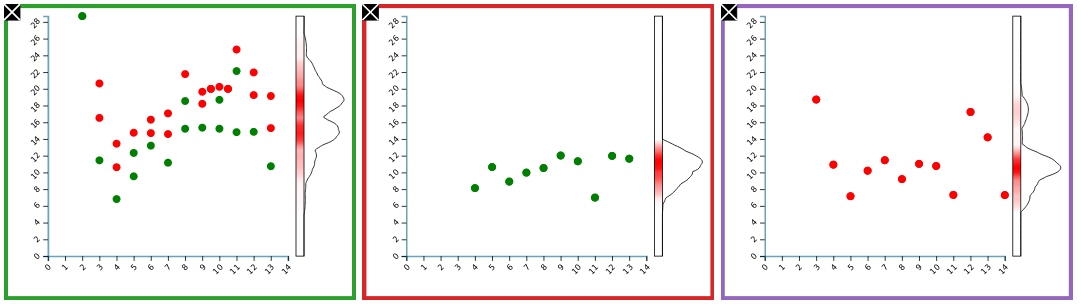
\includegraphics[height=2.35cm]{./img/fview_davg_post.png}
  }

\end{frame}

\begin{frame}{Detail Views -- KDE}

  \begin{block}{Gaussian Kernel (varying length-scales):}

  \centerline{
  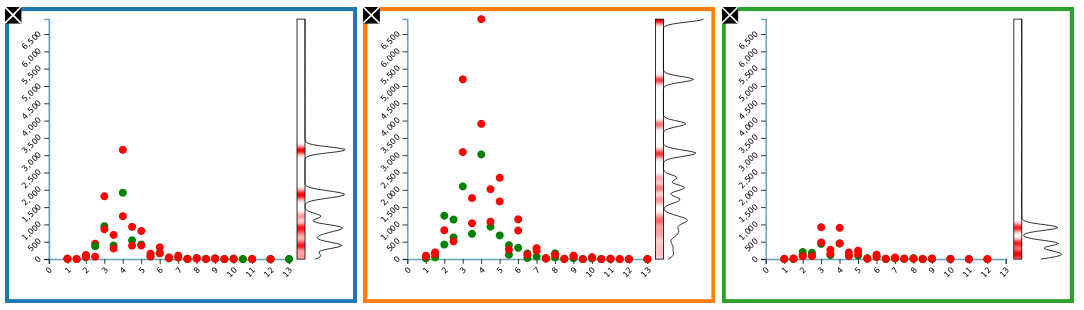
\includegraphics[height=2.35cm]{./img/fview_kde_1.png}
  }

  \centerline{
  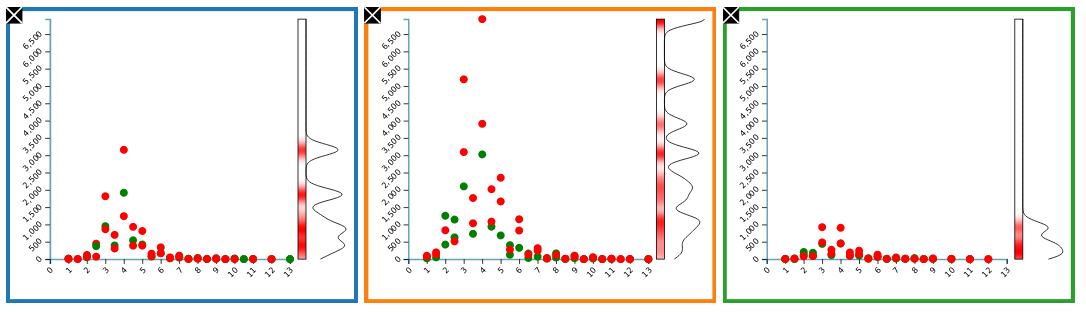
\includegraphics[height=2.35cm]{./img/fview_kde_2.png}
  }

  \centerline{
  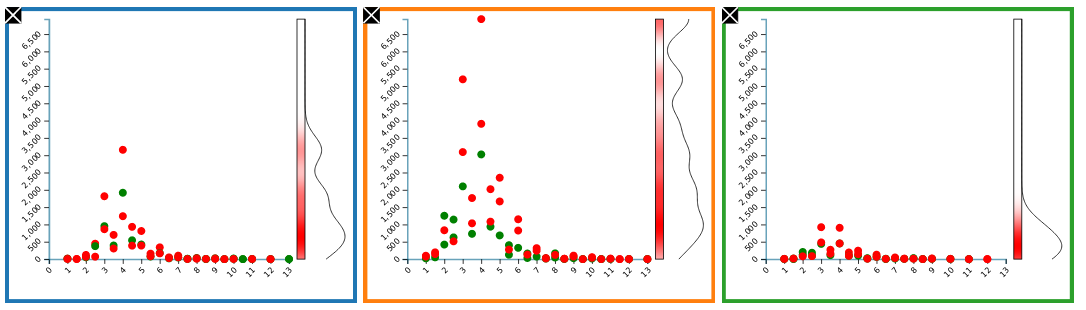
\includegraphics[height=2.35cm]{./img/fview_kde_3.png}
  }

  \end{block}

\end{frame}

\begin{frame}{Detail Views -- GP Regression}

  \begin{block}{Gaussian Kernel:}

  \centerline{
  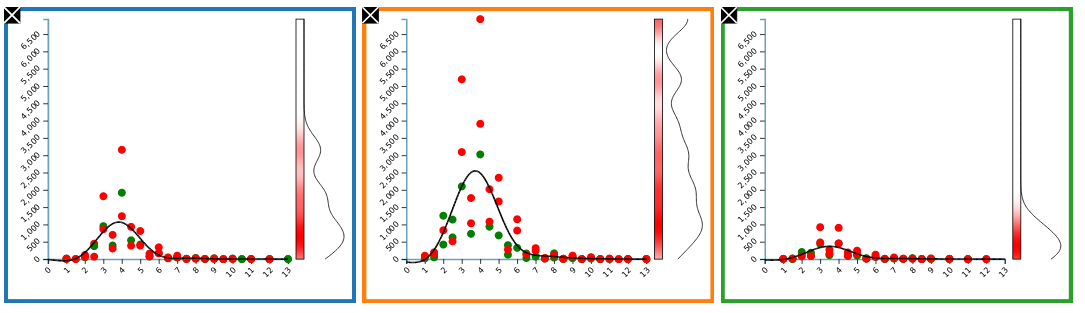
\includegraphics[height=2.35cm]{./img/fview_gp_1.png}
  }

  \end{block}

  \begin{block}{Locally Periodic Kernel:}

  \centerline{
  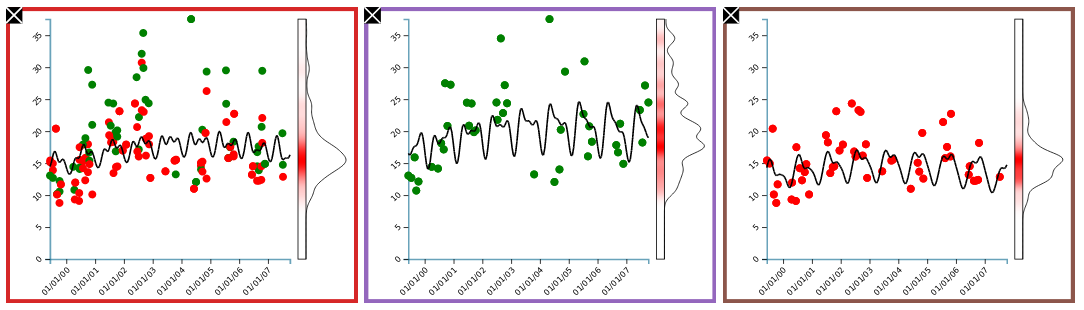
\includegraphics[height=2.35cm]{./img/fview_gp_periodic_1.png}
  }

  \end{block}

\end{frame}

\section*{Live Demo}

\section{Conclusions}

\begin{frame}{Conclusions}

  \begin{block}{Achieved Design Goals}

    \begin{itemize}

      \item Efficient taxonomy navigation and selection.

      \item Axis manipulation aids exploration of relationships within- and
        between- detail view.

      \item Basic ML analysis.

    \end{itemize}

  \end{block}

  \begin{block}{Future Work}

    \begin{itemize}

      \item Improve data fields and data server efficiency.

      \item Switch from Google Maps to lighter d3-geo solution.

      \item Extend data-dim / axis manipulation.

      \item Better management of combined filters.

    \end{itemize}

  \end{block}

\end{frame}

\section*{Questions ?}

\begin{frame}[shrink=10]{Questions?}

  \printbibliography

\end{frame}

\end{document}
